\documentclass[examenvragen.tex]{subfiles}

\begin{document}

\section{Matrix met dominante eigenwaarde}
\subsection{Opgave}
Gegeven de bijgevoegde Maple worksheet. Verklaar de grafieken. Wat is de orde van convergentie en de convergentiefactor? Wat zou er egebeuren als we in de methode geen normalisatie zouden gebruiken?

\subsection{Informatie}
\begin{itemize}
\item Boek pagina 287: Hoofdstuk 6 Het berekenen van eigenwaarden.
\item Boek pagina 290: Opmerking 5 (normalisatie)
\item Boek pagina 292: 6 Slotbemerkingen en samenvatting puntje 5 (convergentie- orde en factor)
\end{itemize}
\subsection{Antwoord}
In de Maple worksheet wordt de methode van de machten (met normalisatie) uitgevoerd op een matrix $A$ met een beginvector $x_0$
\[
A=
\begin{pmatrix}
9 & 1 & -1\\
0 & 10 & -5\\
0 & 0 & 8
\end{pmatrix}
\text{ en }
x_0 = \begin{pmatrix}
-1\\1\\1
\end{pmatrix}
\]
\[
x_{k} = A^{k}x_{0} 
\]
We berekenen eerst de eigenwaarden en eigenvectoren. De eigenwaarden vallen af te lezen op de diagonaal van $A$. Ze zijn re\"el en positief.
\[
\lambda_{1} = 10 \text{ en } E_{1} = \begin{pmatrix}1\\1\\0\end{pmatrix} 
\]
\[
\lambda_{2} = 9 \text{ en } E_{2} = \begin{pmatrix}1\\0\\0\end{pmatrix} 
\]
\[
\lambda_{3} = 8 \text{ en } E_{3} = \begin{pmatrix}-3\\5\\2\end{pmatrix} 
\]
De eigenvectoren vormen een en basis, dus $x_0$ kan uitgedrukt worden als een lineaire combinatie van de eigenvectoren $E_i$ met co\"efficienten $\alpha_i$.
\[
x_{0} = \alpha_{1}E_1 + \alpha_2E_2 + \alpha_{3}E_3
\]
We vinden voor deze $\alpha_i$ de volgende waarden.
\[
\alpha_1 = -\frac{3}{2} \text{, } \alpha_{2} = 2 \text{ en } \alpha_{3} = \frac{1}{2}
\]
Let op: $\alpha_1 \neq 0$. Dit is een voorwaarde om de methode van de machten te kunnen gebruiken. Controleer deze zeker!
We kunnen nu de uitdrukking voor $x_{k}$ uitwerken.
\[
x_{k} = A^{k}x_{0} = A^{k}(\alpha_{1}E_1 + \alpha_2E_2 + \alpha_{3}E_3) = (\alpha_{1}A^{k}E_1 + \alpha_2A^{k}E_2 + \alpha_{3}A^{k}E_3)
= \alpha_{1}\lambda_1^{k}E_1 + \alpha_2\lambda_2^{k}E_2 + \alpha_{3}\lambda_3^{k}E_3)
\]
\[
x_{k} = \lambda_{1}^{k}\left(\alpha_1E_1 + \left(\frac{\lambda_2}{\lambda_1}\right)^{k}\alpha_2E_2 + \left(\frac{\lambda_3}{\lambda_1}\right)^{k}\alpha_3E_3\right)
\]
In deze uitdrukking is $\lambda_{1}^{k}$ duidelijk dominant. Na voldoende iteraties zal er iets overblijven in $x_k$ van de volgende vorm.
\[
x_{k} = \lambda_{1}^{k}\alpha_1E_1 + o(1)
\]
In eerste Maple worksheet, wordt de eigenwaarde iteratief berekend met in de $j$-de iteratiestap $\lambda_{j}$. Dit zal inderdaad naar $\lambda_{1}$ convergeren.
\[
\lambda_{1_{j}} = \frac{\Vert x_{j}\Vert }{\Vert x_{j-1}\Vert}
\]
In de andere Maple worksheet zien we de relatieve fout. Deze verkleint zoals verwacht.

\subsubsection{Convergentiefactor}
De convergentiefactor berekenen we als $\frac{\lambda_{2}}{\lambda_{1}}$
\[
\rho = \frac{9}{10}
\]
We kunnen dit ook uit de grafiek aflezen.
\[
\epsilon_{40} = 10^{-2} \text{ en } \epsilon_{100} = 10^{-6}
\]
De verhouding van de fout in iteratiestap $j$ ten opzichte van de fout in iteratiestap $i$ is (ongeveer) de $j-i$-de macht van $\rho$.
\[
\rho^{100-40} \approx \frac{10_{-6}}{10^{-3}} = 10^{-3}
\]
\[
\rho \approx 0.89125
\]
\subsubsection{Convergentieorde}
De convergentiefactor is niet nul, en de fout daalt superlineair, dus de orde van convergentie is $1$. De methode van de machten convergeert lineair. Dit staat trouwens letterlijk in het boek op pagina 293.

\subsubsection{Zonder normalisatie}
Zonder normalisatie zou $x_{k}$ groeien als $O(n^{k})$. Dit zou vroeg of laat overloop met zich meebrengen. Dan valt er niets meer te zeggen over $\lambda_{1}$. Met normalisatie heeft $x_{k}$ steeds een lengte van $1$.


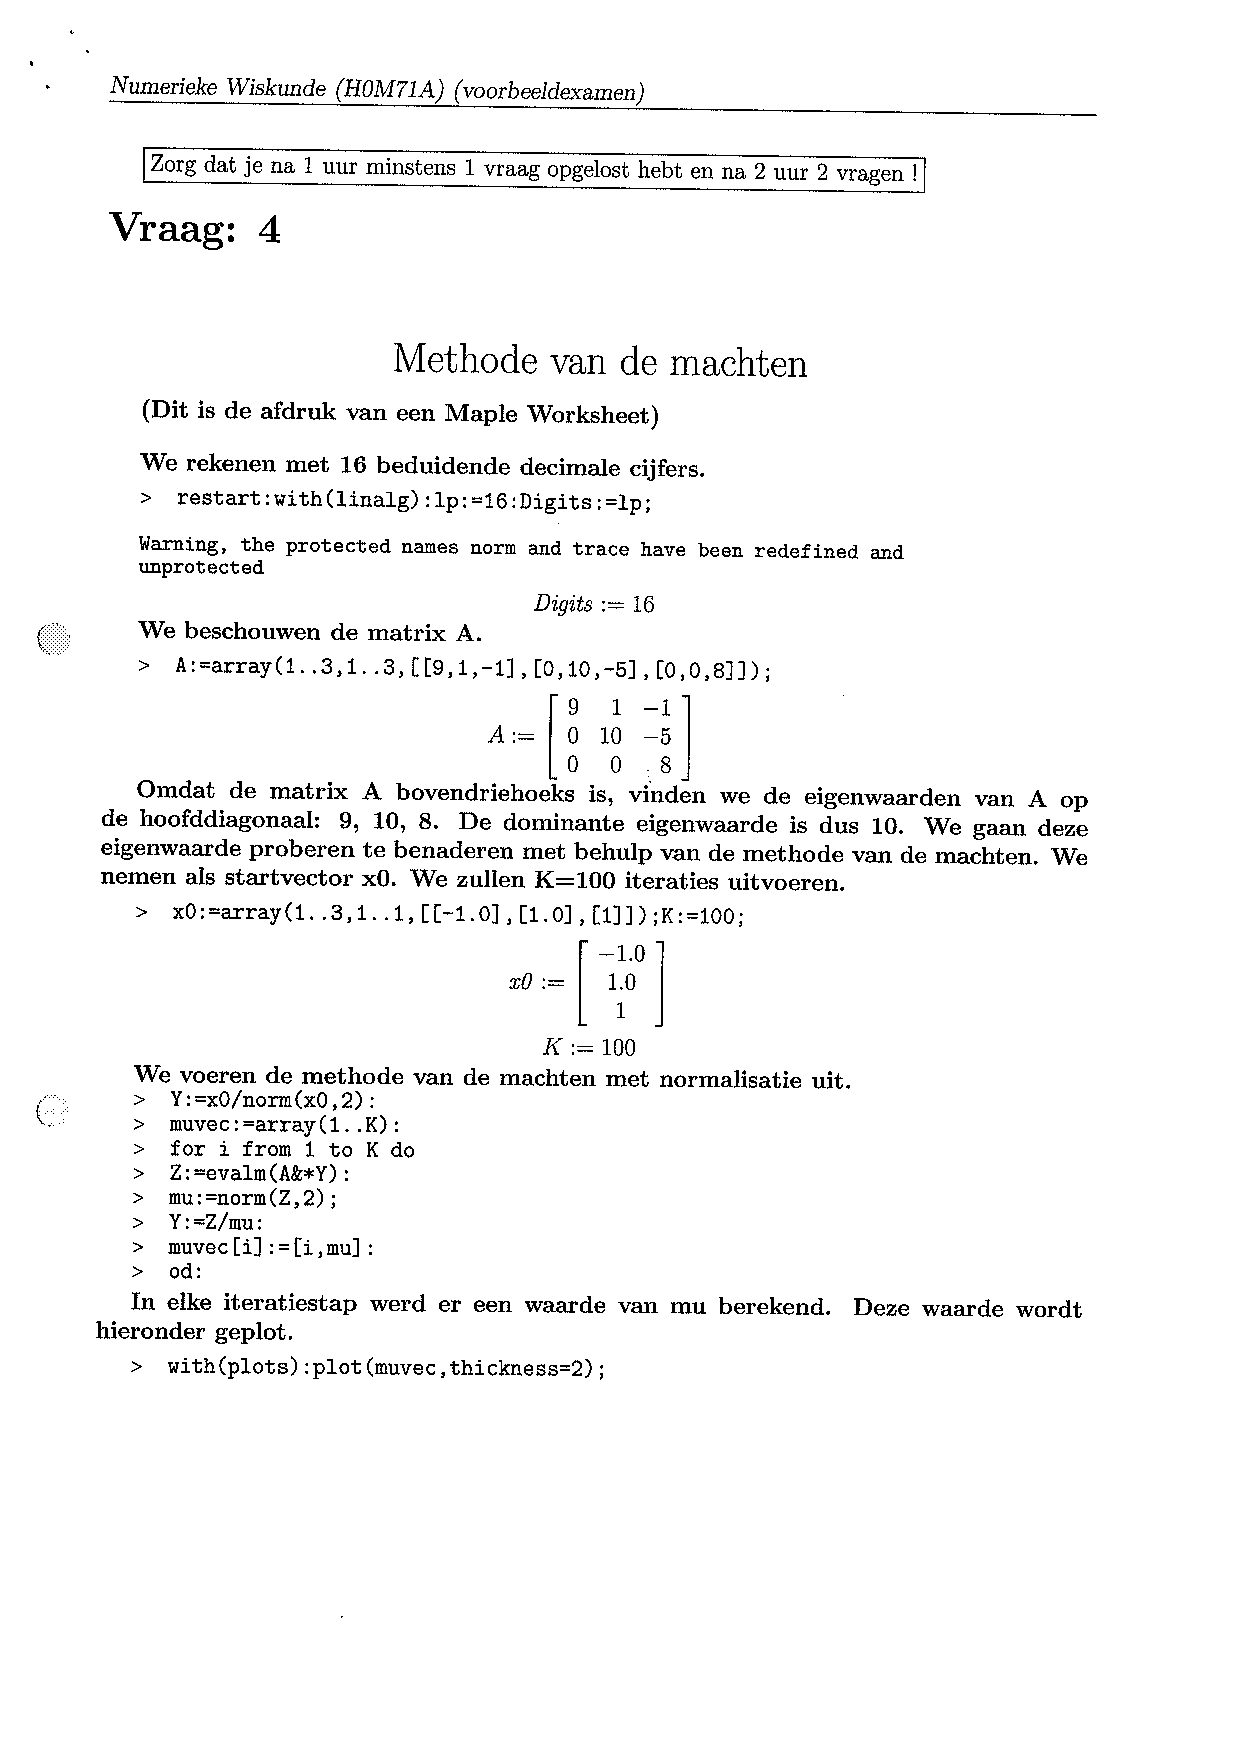
\includepdf[pages=-]{illustraties/vraag_matrix_met_dominante_eigenwaarde_maple_printout.pdf}
\end{document}
